%% IMPORTANT: Once working, run latex 3 times to get listoffigures to work

%% Be sure to check spelling!

%% Put **your** name and the proper due date in place

%% Copy the lstlisting and figure code as many times as you need
%% Be sure to put in your own file names if appropriate

%% Note that the \epsfig commands are currently commented out - until the
%%%% files exist, processing this code without them will result in an error
%%%% so leave the comments until you have created the graphics files!

\documentclass{article}
\usepackage{amsmath}    % load AMS-Math package
\usepackage{epsfig}     % allows PostScript files
\usepackage{listings}   % allows lstlisting environment
\usepackage{moreverb}   % allows listinginput environment
\usepackage{vmargin}    % allows better margins
\setpapersize{USletter} % sets the paper size
\setmarginsrb{1in}{0.5in}{1in}{0.2in}{12pt}{11mm}{0pt}{11mm} %sets margins 
\begin{document}
\begin{center}
\rule{6.5in}{0.5mm}\\~\\
{\bf \large EGR 103L -- Fall 2016}\\~\\
{\huge \bf Laboratory 4 - Loops and Plots}\\~\\
CEMAL YAGCIOGLU (cy111)\\
Lab Section EGR 103L9-05, WEDNESDAY 11.45 PM - 2.35 AM\\
2 OCTOBER, 2016\\~\\
{\small I understand and have adhered to all the tenets of the Duke
  Community Standard in completing every part of this assignment.  I
  understand that a violation of any part of the Standard on any part
  of this assignment can result in failure of this assignment, failure
  of this course, and/or suspension from Duke University.} 
\rule{6.5in}{0.5mm}\\
\end{center}
\tableofcontents
\listoffigures
\pagebreak


%%
\section{Palm Figure 6.1-2}
% Use the code \cite[p.~265]{Palm} somewhere in a line or two about
% how you made the figure
I gave x equally spaced values between 0 and 4 by using linspace code. Then I graphed \begin{align} y=x^m \end{align} (\cite[p.~265]{Palm} for different values of m(-0.5,0,0.5,1,2). I labeled each curve for different values of m with the m value, and gave title to the plot.


\section{Chapra Problem 3.5}
% Compare and contrast the different ways this program worked with angles.
For the Chapra Problem 3.5, my program worked with different values of angle. With increasing number of N(number of steps used in Taylor Series), the accuracy for the given angle increased. On the other hand, with increasing angles, the accuracy of approximations decreased meaning the error increased. Even if the angles are actually are same, meaning two pi subtracted from the angle is same, bigger corresponding angle gave a higher error.
\section{Chapra Problem 4.1}
% Introduction to the table, including a citation, here,
Table of Maclaurin series \cite[p.~120]{Chapra} is; 
% followed by
\begin{center}
{\tt

\begin{tabular}{|ccc|ccc|}\hline 
$a$ & $\epsilon_s$ & maxit & $\sqrt{a}$ & $\epsilon_a$ & iter\\ \hline 
      16 &    1e-02 &        5 & 4.002257524798522e+00 & 3.36e+00 &        5 \\
      16 &    1e-02 &       12 & 4.000000000000051e+00 & 1.59e-05 &        7 \\
      16 &    1e-08 &        5 & 4.002257524798522e+00 & 3.36e+00 &        5 \\
      16 &    1e-08 &       12 & 4.000000000000000e+00 & 1.27e-12 &        8 \\\hline 
     160 &    1e-02 &        5 & 1.482664109800340e+01 & 5.22e+01 &        5 \\
     160 &    1e-02 &       12 & 1.264911068004731e+01 & 7.89e-03 &        8 \\
     160 &    1e-08 &        5 & 1.482664109800340e+01 & 5.22e+01 &        5 \\
     160 &    1e-08 &       12 & 1.264911064067352e+01 & 0.00e+00 &       10 \\\hline 
    1600 &    1e-02 &        5 & 1.052575377021292e+02 & 9.25e+01 &        5 \\
    1600 &    1e-02 &       12 & 4.000000000060651e+01 & 5.51e-04 &       10 \\
    1600 &    1e-08 &        5 & 1.052575377021292e+02 & 9.25e+01 &        5 \\
    1600 &    1e-08 &       12 & 4.000000000000000e+01 & 1.52e-09 &       11 \\\hline 
   16000 &    1e-02 &        5 & 1.005306930179416e+03 & 9.92e+01 &        5 \\
   16000 &    1e-02 &       12 & 1.264911064067374e+02 & 1.86e-05 &       12 \\
   16000 &    1e-08 &        5 & 1.005306930179416e+03 & 9.92e+01 &        5 \\
   16000 &    1e-08 &       12 & 1.264911064067374e+02 & 1.86e-05 &       12 \\\hline 
  160000 &    1e-02 &        5 & 1.000531194227066e+04 & 9.99e+01 &        5 \\
  160000 &    1e-02 &       12 & 4.000285706905372e+02 & 1.20e+00 &       12 \\
  160000 &    1e-08 &        5 & 1.000531194227066e+04 & 9.99e+01 &        5 \\
  160000 &    1e-08 &       12 & 4.000285706905372e+02 & 1.20e+00 &       12 \\\hline 
\end{tabular}

}
\end{center}
% Followed by commentary here about the relative quality of the approximations
The quality of approximations increases as the iteration number increase. For the given iteration number, smaller values of \textit{a} have higher quality of approximations. This can also be observed from increasing number of iterations as \textit{a} increases. While for small values of \textit{a} expected accuracy can be reached before iterations have reached to their maximum value, for higher values of \textit{a} iterations reaches the maxvalue before they can reach to expected accuracy.

\section{3D Projections}
% I figured this one would leave you speechless! Nothing else to say...
The figure and codes are in the appropriate appendices.

\section{Data Logger}
% Still speechless!
The diary, data file, and code are in the appropriate appendices.
\pagebreak

\appendix
\section{Codes}
% Put the name of your file in the subsection name 
% and the listinginput input
% Be sure to include the community standard in codes!
% Add \pagebreaks if they make sense

% Put the files in the same order as the problems; generally, 
% scripts will come first followed by any functions called
% by those scripts.

% Put a \pagebreak after all the scripts/functions
\subsection{ExponentialsGraph.m}
\listinginput[1]{1}{ExponentialsGraph.m}
\subsection{CosSeries.m}
\listinginput[1]{1}{CosSeries.m}
\subsection{DivAvg.m}
\listinginput[1]{1}{DivAvg.m}
\subsection{ThreeDProjections.m}
\listinginput[1]{1}{ThreeDProjections.m}
\pagebreak

\section{Diary and Data Sets}
% This part is already done for you
\subsection{MyTemps.txt}
\listinginput[1]{1}{MyTemps.txt}

\subsection{TempDiary.txt}
\listinginput[1]{1}{TempDiary.txt}
\clearpage

\section{Figures}
% Use [htb!] for plots that show up on first and last page of plots
% Use [htb!p] for plots on the second to penultimate page of plots

% Put a \clearpage after all the plots

\begin{figure}[htb!p]
\begin{center}
%\epsfig{file=FILE.eps, height=3.5in}
%\caption{CAPTION}
\end{center}
\end{figure}

%% This one should be a little bigger...
\begin{figure}[htb!]
\begin{center}
%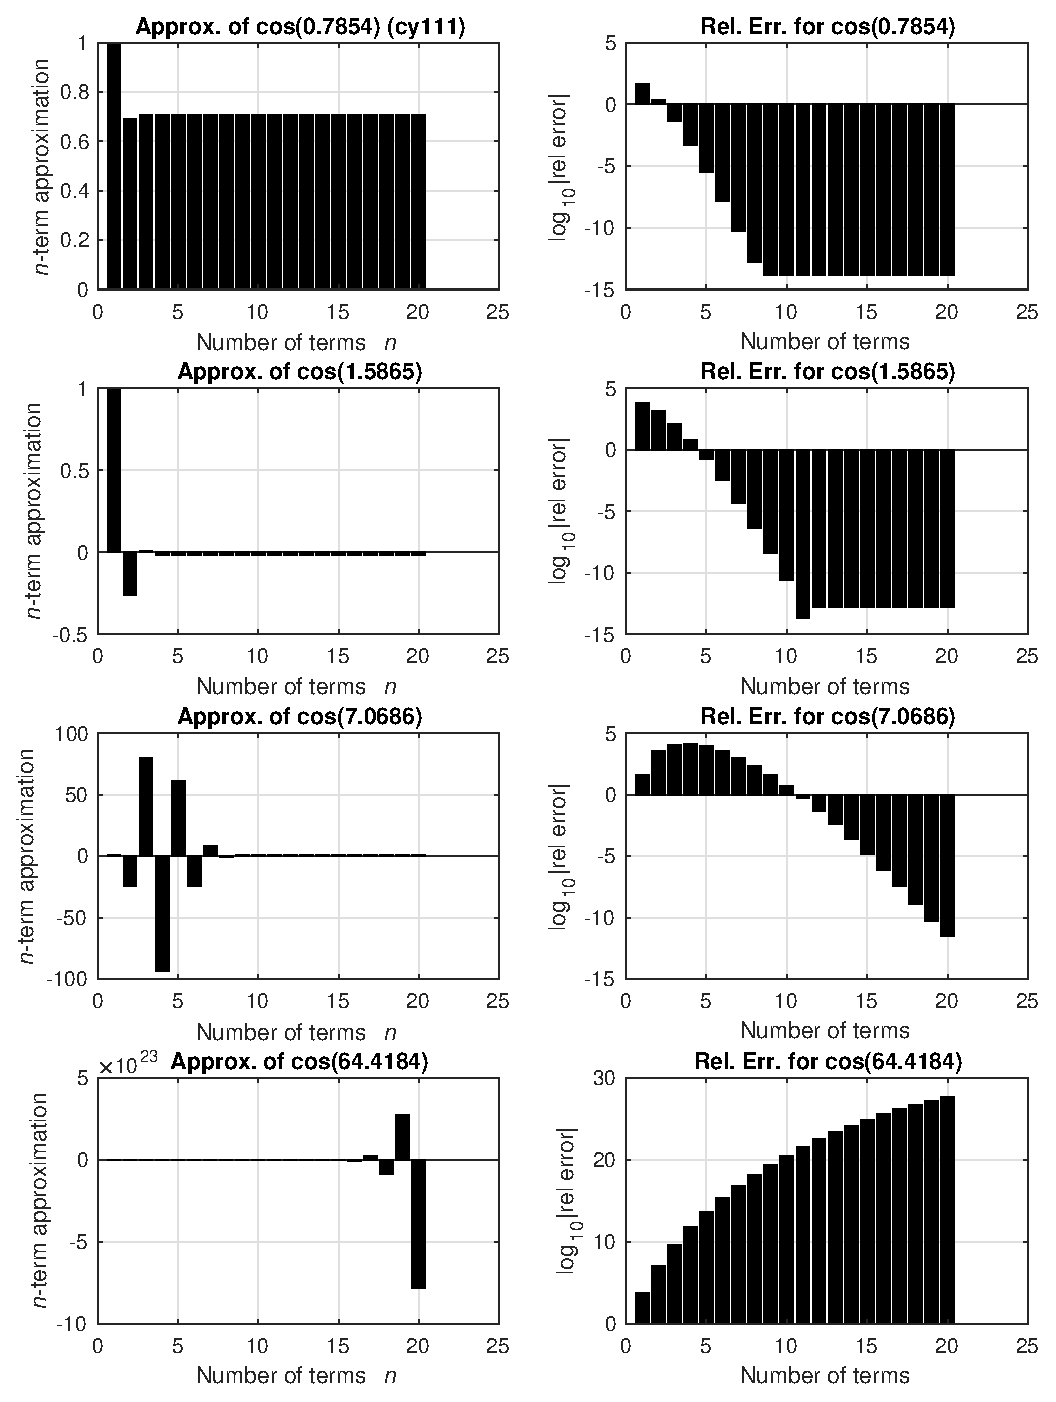
\epsfig{file=CosSeriesCheckerPlot.eps, width=6in}
\caption{Output of {\tt CosSeriesChecker.m} for Chapra 3.5}
\end{center}
\end{figure}

% Other plots...

\clearpage

\begin{thebibliography}{9}
% You're welcome
\bibitem{Chapra}
  Chapra, Steven C.,
  {\it Applied Numerical Methods with MATLAB for Engineering and Scientists}.
  McGraw-Hill, New York,
  3rd Edition,
  2012.
\bibitem{Palm}
  Palm, William J.,
  {\it Introduction to MATLAB for Engineers}.
  McGraw-Hill, New York,
  3rd Edition,
  2011.
\end{thebibliography}

\end{document}



